\documentclass[a4paper,parskip=half]{scrartcl}

\usepackage[T1]{fontenc}
\usepackage[ngerman]{babel}
\usepackage{csquotes}
\usepackage[regular,condensed,sfdefault]{roboto}
\usepackage{graphicx}
\usepackage{chemformula}
\usepackage{amsmath,amsfonts,amssymb}
\usepackage[italic,symbolgreek]{mathastext}
\usepackage[backend=biber]{biblatex}
\usepackage[hidelinks,pdfencoding=auto,
  pdfauthor={Thomas Ascher},
  pdfusetitle,
  pdfkeywords={Bier,Kegging,Zapfanlage}]{hyperref}
\usepackage{microtype}

\addto\extrasngerman{
\def\figureautorefname{Abb.}
}

\addto\captionsngerman{
\renewcommand{\figurename}{Abb.}
}

\title{Alkoholmessung mit dem Refraktometer}
\author{Thomas Ascher}

\addbibresource{refraktometer.bib}

\begin{document}
\maketitle

\section*{Einleitung}

\autocite{Terrill2013}
\autocite{Novotny2017}
\autocite{Novotny2017a}
\autocite{Bonham2001}
\autocite{Gossett2012}
\autocite{Gossett2012a}
\autocite{Gossett2012b}
\autocite{Gossett2012c}
\autocite{Troester2012}
\autocite{Terrill2010}
\autocite{Terrill2010a}
\autocite{Terrill2011}
\autocite{Siebel1938}
\autocite{Weiss2016}
\autocite{BrewersJournal2017}
\autocite{Annemueller2015}
\autocite{Kunze2004}

\newcommand{\rii}{\mathit{R}_i}
\newcommand{\riic}{\mathit{Rc}_i}
\newcommand{\rif}{\mathit{R}_f}
\newcommand{\rifc}{\mathit{Rc}_f}
\newcommand{\fg}{\mathit{FG}}
\newcommand{\abv}{\mathit{ABV}}
\newcommand{\abw}{\mathit{ABW}}

\subsection*{Bonham (2001)}

\begin{align}
\begin{split}
\fg &= 1.001843 - 0.002318474 \cdot \riic - 0.000007775 \cdot \riic^2 -
0.000000034 \cdot \riic^3 \\
& \quad + 0.00574 \cdot \rif +
0.00003344 \cdot \rif^2 + 0.000000086 \cdot \rif^3
\end{split} \label{eq:bonham} 
\end{align}

\begin{align}
\begin{split}
\abv = \frac{(277.8851 - 277.4 \cdot \fg + 0.9956 \cdot \rif + 0.00523 \cdot \rif^2 + 0.000015 \cdot \rif^3) \cdot \fg}{0.79}
\end{split}
\end{align}

\begin{equation}
\mathit{AE}=1.53 \cdot \rif - 0.59 \cdot \riic
\label{eq:gardner} 
\end{equation}

\begin{equation}
\abw = 1.09 \cdot \rif - 1.13 \cdot \mathit{AE}
\end{equation}

\subsection*{Terrill (2011)}

\begin{equation}
\fg = 1 - 0.00085683 \cdot \riic + 0.0034941 \cdot \rifc
\label{eq:terrilllinear} 
\end{equation}

\begin{align}
\begin{split}
\fg &= 1 - 0.0044993 \cdot \riic + 0.011774 \cdot \rifc + 0.00027581 \cdot \riic^2 - 0.0012717 \cdot \rifc^2 \\
& \quad  - 0.0000072800 \cdot \riic^3  + 0.000063293 \cdot \rifc^3
\end{split} \label{eq:terrillcubic} 
\end{align}

\subsection*{Gossett (2012)}

\begin{equation}
k = 0.445
\end{equation}

\begin{equation}
C = 100 \cdot \frac{\rii - \rif}{100 - 48.4 \cdot k - 0.582 \cdot \rif}
\end{equation}

\begin{equation}
\abw = \frac{48.4 \cdot C}{100 - 0.582 \cdot C}
\label{eq:gossett} 
\end{equation}

\subsection*{Novotný (2017)}

\begin{equation} 
\fg = -0.002349 \cdot \riic + 0.006276 \cdot \rifc + 1
\label{eq:novotnylinear} 
\end{equation}

\begin{align}
\begin{split}
\fg &= 1.335 \cdot 10^{-5} \cdot \riic^2 - 3.239 \cdot 10^{-5} \cdot \riic \cdot \rifc + 2.916 \cdot 10^{-5} \cdot \rifc^2 \\
& \quad - 2.421 \cdot 10^{-3} \cdot \riic + 6.219 \cdot 10^{-3} \cdot \rifc + 1
\end{split} \label{eq:novotnyquadratic} 
\end{align}

\begin{equation} 
\abw = 0.67062 \cdot \riic - 0.66091 \cdot \rifc
\end{equation}

\begin{equation} 
\mathit{RE} = -0.29388 \cdot \riic + 1.27582 \cdot \rifc
\end{equation} 

\begin{equation} 
\abv = \frac{\fg \cdot \abw}{0.791}
\end{equation} 


\autoref{eq:novotnylinear}

%(\autoref{fig:groteblohm}) von 
%Grote \& Bohm \autocite{GroteBlohm2020}.

%\begin{figure}[h]
%\centering
%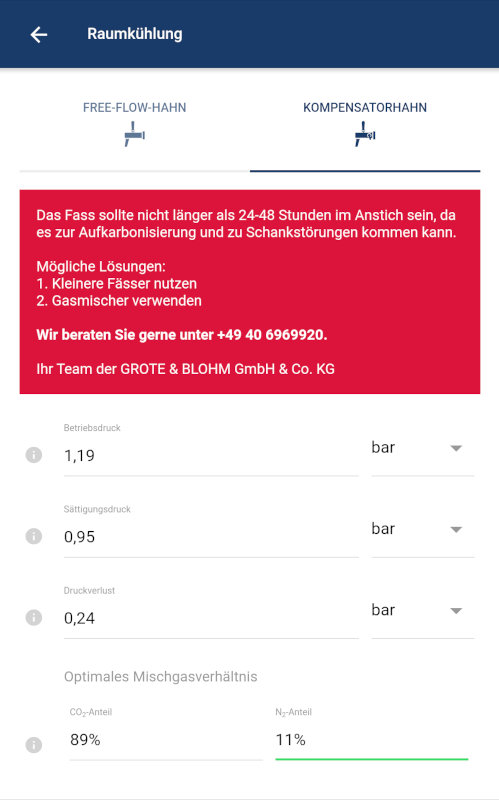
\includegraphics[width=4.8cm]{images/groteblohm.jpg}
%\caption{FOBB-APP}
%\label{fig:groteblohm}
%\end{figure}


\printbibliography[title=Quellen]

\end{document}